%%%%%%%%%%%%%%%%%%%%%%%%%%%%%%%%%%%%%%%%%%%%%%%%%%%
%
%  New template code for TAMU Theses and Dissertations starting Fall 2012.
%  For more info about this template or the
%  TAMU LaTeX User's Group, see http://www.howdy.me/.
%
%  Author: Wendy Lynn Turner
%	 Version 1.0
%  Last updated 8/5/2012
%
%%%%%%%%%%%%%%%%%%%%%%%%%%%%%%%%%%%%%%%%%%%%%%%%%%%
%%%%%%%%%%%%%%%%%%%%%%%%%%%%%%%%%%%%%%%%%%%%%%%%%%%%%%%%%%%%%%%%%%%%%%
%%                           SECTION III
%%%%%%%%%%%%%%%%%%%%%%%%%%%%%%%%%%%%%%%%%%%%%%%%%%%%%%%%%%%%%%%%%%%%%

\chapter{\texorpdfstring{\MakeUppercase{Optimization Methodology}}{Optimization Methodology}}

In order to optimize the system, the energy use from each of the components
comprising the air-side equipment needs to be estimated. This includes fan
energy, cooling energy, and reheat energy.

Fan Energy:
\begin{equation} \label{eq:FanEqnergy}
\dot E_{fan} = fct\left( {\flow{supply},\Delta {P_{s,{\rm{fan}}}}} \right)
\end{equation}

Cooling Energy:
\begin{equation} \label{eq:CoolingEnergy}
    {\dot E_{cooling}} = {\flow{supply}}\rho_a c_{p,a}\:\left( {{T_{ma}} - {\sat}} \right) + h_v\rho_a{\flow{supply}}\:\left( {{\omega _{ma}} - {\omega _{sa}}} \right)
\end{equation}

\section{Reheat in Terminal Units}

Terminal units can be distributed into 3 classifications for this work.
Terminal units with no fans, series flow, or parallel flow arrangements.

\subsection{No Fan in Terminal Unit}

If there is no fan and only a damper for air volume modulation, then the reheat
energy use is

\begin{equation} \label{eq:ReheatEnergy}
    {\dot E_{reheat}} = \sum\limits_i {{\flow{i}}\rho_a c_{p,a}\:\left( {{T_{i,dis}} - {T_{i,sa}}} \right)}
\end{equation}

\subsection{Series Flow Configuration}

For a series flow terminal unit, the total flow is ideally constant.
\(\flow{tot}\) is known from specification of the terminal unit and
\(\flow{pri}\) is a measured variable. \(\flow{plen}\) can be calculated from
Eq. (\ref{eq:TotalFlow}).

%-------------------------------------------------------------------------------------------
\begin{figure}
\centering
\begin{tikzpicture}
\begin{axis}[
	xmin=0,
    xmax=100,
    ymin=0,
    ymax=120,
	grid=major,
	ylabel = {Percent Design CFM},
	%height=9cm,
    xtick=\empty,
    ytick={0,25,...,100},
    ymajorgrids=false,
    clip mode=individual,
]
\addplot[
	no markers,
	mark=o,
    color=black,
    dashed,
]
table[x=RoomConditionsPrimary,y=PercentDesignCFMPrimary,col sep=tab] {SeriesFanPlot.dat};

\addplot[
	no markers,
    color=black,
    solid,
]
table[x=RoomConditionsTotal,y=PercentDesignCFMTotal,col sep=tab]{SeriesFanPlot.dat};


\node at (25,60) {Plenum Air};
\node at (78,20) {Primary Air};
\node at (50,110) {Total Air};
\node [anchor=south west] at (0, -15) {Heating};
\node [anchor=south east] at (100, -15) {Cooling};

\end{axis}
\end{tikzpicture}
\begin{tikzpicture}
\begin{axis}[
	xmin=0,
    xmax=100,
    ymin=50,
    ymax=110,
	grid=major,
	ylabel = {Discharge Air Temperature \(^\circ\)F},
	%height=9cm,
    xtick=\empty,
    ytick={50,60,...,100},
    ymajorgrids=false,
    clip = false,
    clip mode=individual,
]
\addplot[
	no markers,
    color=black,
    solid,
]
table[x=RoomTemp,y=Tdischarge,col sep=tab]{SeriesFanPlot.dat};
\node [anchor=south west] at (0, -60) {Heating};
\node [anchor=south east] at (100, -60
) {Cooling};
\end{axis}
\end{tikzpicture}
\caption{Example Series Terminal Unit Flow Operation}
\label{fig:SeriesFlow}

\end{figure}
%-------------------------------------------------------------------------------------------


\begin{equation} \label{eq:TotalFlow}
    \flow{plen} = \flow{tot} - \flow{pri}
\end{equation}

\(T_{dis}\) will be sensed. The temperature of the air after mixing can be
estimated from the flow information and an assumption or measurement of plenum
air.

\begin{equation} \label{eq:MixedAirTemperature}
\mat = \frac{{{\priflow}\left( {\sat} \right) + \plenflow \left( {{T_{plen}}} \right)}}{\totflow}
\end{equation}

Another rearrangement of \ref{eq:MixedAirTemperature} that is important is
solving for \(\flow{pri}\). Under conditions when there is no reheat and the
primary flow is not at the minimum setting, the energy balance across the
terminal unit is

\begin{equation}
    \priflow \sat + \plenflow T_{plen} = \totflow \dat
\end{equation}
Replacing \(\plenflow{} \) with \eqreftext{} \ref{eq:TotalFlow} gives
\begin{equation}
    \priflow \sat +  \left(\totflow - \priflow \right)  T_{plen} = \totflow \dat
\end{equation}
\begin{equation}
 \totflow T_{plen}  -   \totflow \dat  = \priflow  T_{plen}  - \priflow \sat
\end{equation}
\begin{equation}\label{eq:priflowWithoutReheat}
   \priflow = \totflow \left( \frac{T_{plen} - \dat }{T_{plen} - \sat} \right)
\end{equation}

The actual primary flow will be the maximum of \eqreftext{}
\ref{eq:priflowWithoutReheat} and the minimum flow setting. When at minimum
flow, there will be resulting reheat.


\begin{equation} \label{eq:PrimaryFlowInTerminalUnit}
    \priflow = \text{MAX}\left(\frac{\totflow \left(T_{dis} - T_{\plenum} \right)}{\left(T_{\primary} - T_{\plenum} \right)}, \flow{\primary, \text{min}} \right)
\end{equation}


The increase in temperature to the discharge temperature is due to heat gain
from the fan and from any supplementary heating.

The temperature rise from the fan, \(\Delta T_{fan}\), can be estimated from
historical data when the supplementary heating is off, either when the heating
coil is completely closed or all stages of electrical reheat are inactive. If
there is no other heating, the temperature increase from the fan is

\begin{equation}
\Delta {T_{fan}} = {T_{dis}} - {T_{mix}}.
\end{equation}
%
For other times, the temperature increase due to reheat will be
%
\begin{equation}
\Delta {T_{reheat}} = {T_{dis}} - \left( {\Delta {T_{fan}} + {T_{mix}}} \right),
\end{equation}
%
and the reheat energy will be
%
\begin{equation}
{\dot Q_{reheat}} = {\dot V_{tot}}{\rho _a}{c_{p,a}}\left( {\Delta {T_{reheat}}} \right).
\end{equation}

\subsection{Parallel Flow Configuration}

During periods of cooling, the fan in a parallel arrangement is off and the
total flow is equal to the primary flow.

The fan volume flow will be known from manufacturers specifications and the
total flow can be calculated using Eq. \eqref{eq:TotalFlow}. The temperature
from mixing the plenum air and primary can be estimated from Eq.
\eqref{eq:MixedAirTemperature} or from historical data when the primary flow is
at the minimum and there is no activated reheat components.

\subsection{Other Terminal Unit Types}

Terminal units come in even more configurations than the three specified
in this document, induction units being one example. Models can be made
using a combination of energy balances, historical data under particular
conditions, and appropriate assumptions.

\section{Required Sensors}

In order to fulfill the proposed methodology, there are several sensors that
are not common that would need to be installed.

\tableref{} \ref{tab:NecessarySensors} lists the minimum set of sensors
required. The sensors that are least likely to be available are the static
pressure at the fan and the discharge air temperature from each terminal
unit.

\begin{table}
\centering
\begin{tabular}{l l}
\toprule

Level & Sensor \\
\midrule\midrule
\multirow{2}{*}{Weather} & Outdoor Air Temperature \\
 & Outdoor Dew Point Temperature \\

 \midrule

\multirow{6}{*}{AHU}              & Supply Air Temperature      \\
                                  & Mixed Air Temperature       \\
                                  & Fan Power                   \\
                                  & VFD Command                 \\
                                  & Static Pressure at Fan      \\
                                  & Static Pressure for Control \\
\midrule
\multirow{4}{*}{Terminal Units}   & Primary Air Flow Rate       \\
                                  & Discharge Air Temperature   \\
                                  & Primary Damper Position     \\

\bottomrule

\end{tabular}
\caption{Necessary Sensors}
\label{tab:NecessarySensors}
\end{table}

\section{Predicting Zone Loads}

The zone loads can be estimated from terminal unit data of airflow rate,
terminal unit leaving temperature and zone temperature. Note that using
%
\begin{equation}
\dot Q_{zone} = \dot V_{zone} C_{air} \left(T_{zone}-T_{leaving} \right)
\end{equation}
%
assumes that the space is well-mixed and at steady-state. If the controls
oscillate, then the zone load estimation will have some periodicity. In one
sense, there is no ``single'' zone load coming from a point source, and as such
we will have to rely on this estimation.

The independent variables available for prediction are the current time and
outdoor air conditions. The current time can be separated into time of day, day
of week, weekdays/weekends and such. Outdoor air temperature correlates with
the external load. As a reminder, this approach does not have access to live values
of sensors and only relies on historical data.

The approach used to estimate parameters is a related to the concept of
a \textit{nearest neighbor}. The nearest neighbors are defined by any
previous data that:

\begin{enumerate}
    \item Was within \(n\) hours of the time of day, normally taken as plus or minus one time step.
\item Was the same day of the week
\item Had a corresponding \(T_{db}\) that is within \(\pm 2.5^\circ\)F of the the current \(T_{db}\).
\end{enumerate}

The median value of the nearest neighbors can be used to estimate the
particular zone load at any time and temperature.  The median is a more robust
statistic in comparison to the mean, having a breakdown point of 50\%, meaning
that up to 50\% of the data can be contaminated before the median statistic
will no longer be reliable. For the mean, one arbitrarily large data point can
turn the mean statistic unreliable.

This work used the most recent 30 data points in the median calculation. 30 points
was chosen since this is the threshold in which the sample median should approximate
the actual median, if the population is assumed to have a normal distribution.

It is advised that in this approach, that the initial historical data be sorted
in order of temperature, followed by the date time.  The lookup for the
subsection of data to be used will then be \(O\left(\log n \right)\) with a
binary lookup.

The advantage of the nearest neighbor approach is that the resulting ``function''
is not limited to being linear, quadratic, or any particular form. It just
simply matches the data as best it can during external conditions that are
expected to be similar.

\subsection{Zone Load Uncertainty}

The Kline-McClintock form of uncertainty analysis can be applied to the
zone loads.

If the zone load is described as an open system with a constant specific
heat, then
\begin{equation}
    \dot{Q}_{zone} = 60 \frac{\flow{zone}}{\nu} c_{air} \left(T_{room} -
    T_{sup}\right)
\end{equation}
where \(\flow{zone}\) is in units of CFM, \(\nu\) is in
\si{\feet\cubed\per\pound}, \(c_{air}\) is in
\si{\btu\per\pound\per\degreeF}, the temperatures are in
\si{\degreeF}, and the zone load is in \si{\btu\per\hour}.

The total uncertainty in the prediction will be
\begin{equation}
\small
    \delta \dot{Q}_{zone} = 60\,c_{air} \sqrt{ \left( \frac{\left(T_{room} - T_{sup}\right)}{\nu} \delta \flow{} \right)^2 
    + \left( \frac{- \left(T_{room} - T_{sup}\right) \flow{}}{\nu^{2}} \delta \nu \right)^{2}  
+ \left( \frac{\flow{}}{\nu} \delta T_{room}\right)^{2}
+ \left(\frac{-\flow{}}{\nu} \delta T_{sup}\right)^{2}
}
\end{equation}
For the sake of analysis, the following parameters were assumed:
\begin{enumerate}
    \item \(T_{room} = \SI{72}{\degF} \)
    \item \(T_{sup} = \SI{55}{\degF} \)
    \item \(\nu = \SI{13.5}{\feet\cubed\per\poundMass}\)
    \item \(\delta T_{room} = \delta T_{sup} = \SI{1}{\degF}\)
    \item \( \delta \nu = \SI{1}{\feet\cubed\per\poundMass} \)
\end{enumerate}

The resulting percent uncertainty in the zone load versus the
uncertainty in the flow measurement is shown in \figref{}
\ref{fig:ZoneLoadUncVsFlowUnc}. To note is that with no flow
uncertainty, there is approximately 11\% percent uncertainty
contribution from the air density and temperatures. After about 20\%
uncertainty in the flow, it becomes the dominant source of uncertainty. 


%\begin{equation}
    %\delta \dot{Q}_{zone} = \sqrt{\frac{3600 c^2 {\delta \nu}^2 V^2
    %(T_{room}-T_{zone})^2}{\nu ^4}+\frac{3600 c^2
    %{\delta T_{room}}^2 V^2}{\nu ^2}+\frac{3600 c^2 {\delta T_{sup}}^2
       %V^2}{\nu ^2}+\frac{3600 c^2
       %{\delta \flow{}}^2 (T_{room}-T_{zone})^2}{\nu ^2}+\frac{3600
       %{\delta c}^2 V^2
             %(T_{room}-T_{zone})^2}{\nu ^2}}
%\end{equation}

\begin{figure}
\centering
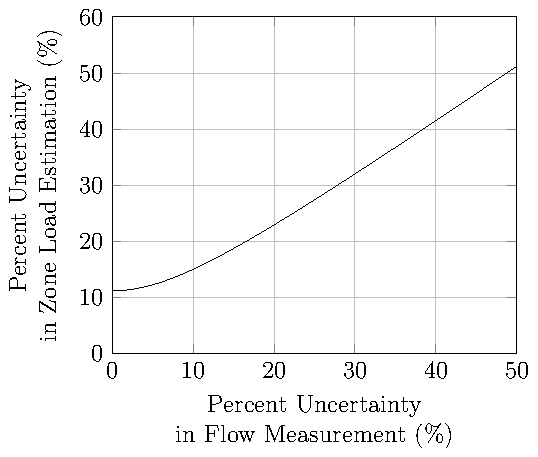
\includegraphics[]{Plots/2017-05-16-ZoneLoadUncertaintyVsFlowUncertainty.pdf}
\caption{Zone load uncertainty versus flow uncertainty.}
\label{fig:ZoneLoadUncVsFlowUnc}
\end{figure}






\subsection{Analysis of Fraction of Full Load Power Uncertainty}
\begin{figure}
\centering
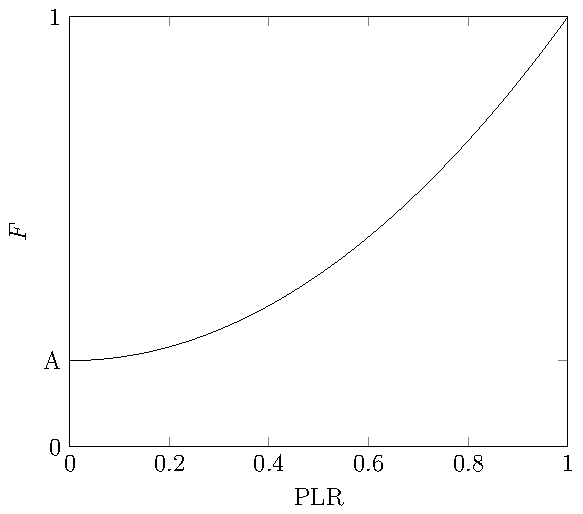
\includegraphics[]{Plots/2017-05-12-Fcurve.pdf}
\caption{Fraction of full load power for a fan.}
\label{fig:FCurve}
\end{figure}

In simplified air handling unit analysis, the fraction of full load
power, \(F\), can often be represented with the function shown in
\figref{} \ref{fig:FCurve}
\begin{equation}
    F = A + (1-A)( \text{PLR} )^{n}
\end{equation}
where \(A\) is the fraction of power at zero load, \(n\) is an exponent
ranging from 1 to 3, and PLR is the part load
ratio defined to be
\begin{equation}
    \text{PLR} = \frac{\flow{act}}{\flow{design}}
\end{equation}
The actual fan power at any point is then
\begin{equation}
    \power{act}  = F \power{design}
\end{equation}
The uncertainty of \(F\) can be explored with the Kline-McClintock
formulation.

The first term related to the uncertainty in \(A\) is
\begin{equation}
A \text{ term} = \pdv{F}{A} \delta A = \left(1-\text{PLR}^n\right) \delta A
\end{equation}
The uncertainty term related to \(n\) is
\begin{equation}
    n \text{ term} = \pdv{F}{n} \delta n = \left((1-A) \text{PLR}^n \ln (\text{PLR})\right) \delta n
\end{equation}
and the uncertainty related to PLR is
\begin{equation}
    \text{PLR term} = \pdv{F}{ \text{PLR}} \delta \text{PLR} = \left((1-A) n \text{PLR}^{n-1}\right) \delta \text{PLR}
\end{equation}
The total uncertainty in \(F\) is
\begin{equation}
    \delta F = \sqrt{ \left(A \text{ term}\right)^{2} + \left(n \text{ term}\right)^{2} + \left( \text{PLR term}\right)^{2} }
\end{equation}
The uncertainty is a function of 6 variables: \(A\), \(n\), PLR, \(\delta A\), \(\delta n\), and \(\delta\)PLR.

If the values of
\begin{enumerate}
    \item \(A=0.2\)
    \item \(n=2\)
    \item \(\delta A = 0.05\)
    \item \(\delta PLR = 0.05\)
    \item \(\delta n = 0.4\)
\end{enumerate}
are used, a plot can be created showing the relative importance in the
uncertainty as a function of PLR. This plot is shown in \figref{}
\ref{fig:FFLRUncertainty}.

Over the input range of PLR, there are three different regimes in which
each input variable contributes the most to the uncertainty. At high
part load ratios, the uncertainty in the part load ratio itself is the
most important factor. At part load ratios near 0.5, the exponent \(n\),
which determines the curvature is the most important. At low part load
ratios, the uncertainty in the value of \(A\), the limiting fraction of
part load power at 0 load, is the most important.

So to reduce the total uncertainty across all ranges of part load ratios
will require better knowledge of all the input variables.

\begin{figure}
\centering
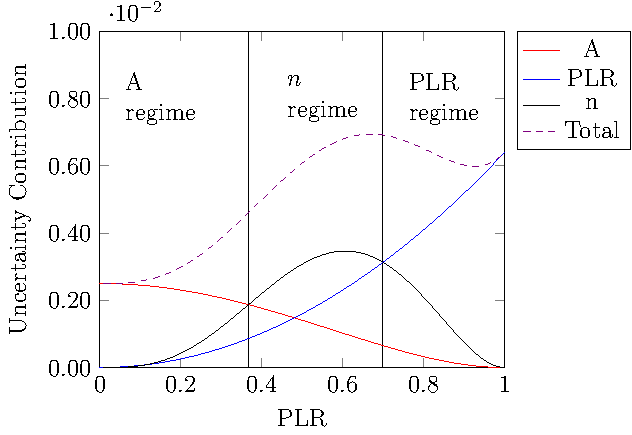
\includegraphics[]{Plots/2017-05-15-FFLPUncertainty.pdf}
\caption{Relative uncertainty contributions for fraction of full load
fan power.}
\label{fig:FFLRUncertainty}
\end{figure}

\figref{} \ref{fig:TotalFFLRUncertainty} shows the total uncertainty in
\(F\), given the assumed inputs listed. At all levels of part load, the
estimated uncertainty in the fraction of full load power is less than
0.1.

If all the individual uncertainties are reduced by half, the total
uncertainty will also be reduced by half. The would be feasible with
trend data regarding the individual fan powers, flow, and pressures.
This would put the maximum uncertainty in \(F\) to about 0.04.

\begin{figure}
\centering
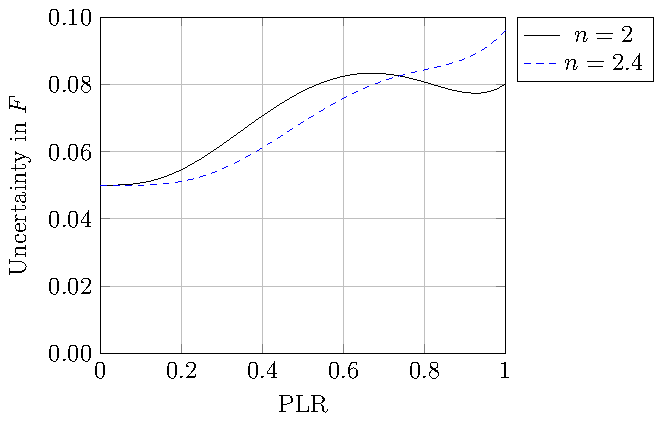
\includegraphics{Plots/2017-05-15-totalFFLPUncertainty.pdf}
\caption{Total uncertainty in the fraction of full load fan power, \(F\).}
\label{fig:TotalFFLRUncertainty}
\end{figure}



%\section{Setup Employing Historical Trend Data}

%Before the system can be run, some of first principles models need to be
%calibrated. The calibration will employ historical measured data.

\section{Fan Modeling}\label{sec:FanModeling}

Fan energy is a significant component to the air side energy use for air
conditioning. Fan static pressure, flow, speed, and power will all be
measured.  The total primary air flow can either be measured directly
(ideal) or estimated from the sum of the children terminal units. With
this information, a complete set of fan curves can be created.

Without all the sensors it's hard to create a first-principle based model
of the air-side equipment. Statistical techniques would be necessary to relate
the speed of the fan, \(\dot N\), and the damper positions,
\(\damp{i,damper}\).

\subsection{Air Distribution Modeling: First Method}
This section is a bit of an aside and is presented to show the negative
result given the following setup.

Estimating the system pressure loss for particular conditions is
necessary for determining the potential fan energy at different speeds.
The node layout of the terminal units will need be created. If the air
flow through each terminal unit is measured the flow through each
portion of the duct work can be estimated.

The first methodology developed attempted to break the air side pressure
drops into parts for the major losses within the duct work and the minor
losses due to the dampers at the terminal unit.

The following assumptions were made:

\begin{itemize}
    \item Constant friction factors
    \item Reference pressure of 0 at each zone
    \item Linear flow response from the damper position
\end{itemize}


\begin{figure}
\centering
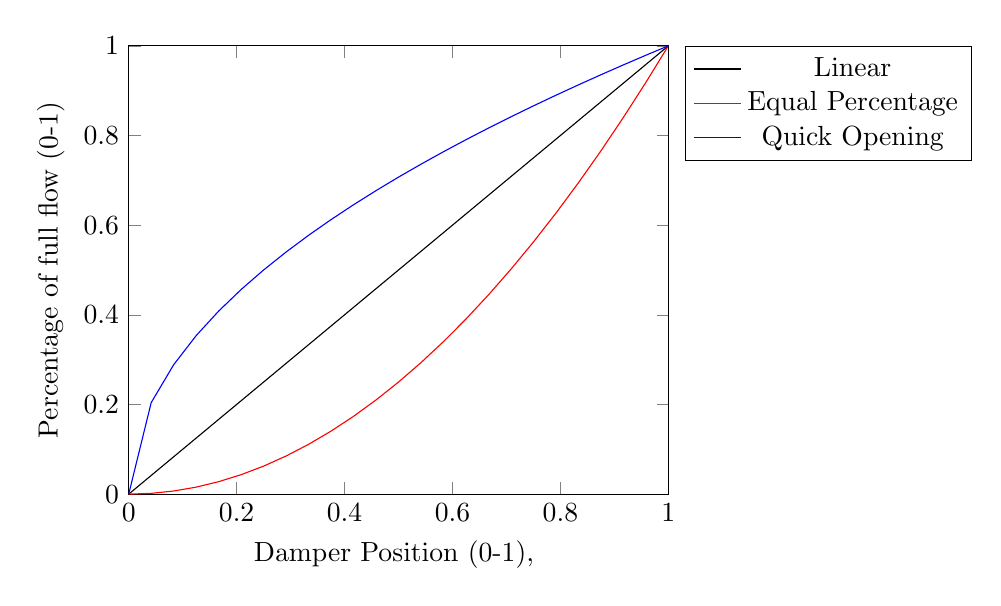
\begin{tikzpicture}
\begin{axis}[
        xmin=0,
        xmax=1,
        ymax=1,
        ymin=0,
        legend pos=outer north east,
        xlabel={Damper Position (0-1), \(\damp{}\)},
        ylabel={Percentage of full flow (0-1)},
    ] \addplot[
        domain=0:1,
        black,
    ]
    {x};

    \addlegendentry{Linear}

    \addplot[
        domain=0:1,
        red,
    ]{x*x};
    \addlegendentry{Equal Percentage}
\addplot[
        domain=0:1,
        blue,
    ]{sqrt(x)};
    \addlegendentry{Quick Opening}
\end{axis}
\end{tikzpicture}
\caption{Terminal unit flow response as a function of damper position.}
\label{fig:flowVersusDamperPos}
\end{figure}



With the assumption of the constant friction factor, the pressure drop
in each duct section will be proportional to a constant and the flow
through the section squared. Figure \ref{fig:flowVersusDamperPos} shows
the typical types of responses for a damper or valve.

\begin{equation}\label{eq:PressureDrop}
    \Delta P_{\text{fan}} = C\left(\flow{t}\right)^2
\end{equation}

If \(\flow{t}\) is reduced to some percentage of full flow, then
\eqreftext{} \ref{eq:PressureDrop} will result in
 \begin{equation}
     C = \frac{\Delta P_{\text{fan}}}{\left( \flow{t} \cdot \%_{\text{full flow}} \right)^2}
 \end{equation}

For a linear response

\begin{equation}
    \%_{\text{full flow}} = \damp{}
\end{equation}
and therefore the local loss coefficient \(C\) equals
\begin{equation}
C = \frac{\Delta P_{\text{fan}}}{\left( \flow{t} \cdot \damp{}  \right)^2}
\end{equation}
and grows as a function of \(1/x^2\).

At any time, the pressure drop in all the flow loops must be equal. In a
case where there are three terminal units, you would end up with
relationships like the following

\begin{align}
    \Delta P_{fan}  &= C_1 \left(\flow{1}+\flow{2}+\flow{3} \right)^2 + \frac{C_2}{\damp{1}^2}\flow{1}^2 \\
                    &= C_1 \left(\flow{1}+\flow{2}+\flow{3} \right)^2 + C_3\left(\flow{2}+\flow{3} \right)^2 + \frac{C_4}{\damp{2}^2}\flow{2}^2 \\
                    &= C_1 \left(\flow{1}+\flow{2}+\flow{3} \right)^2 + C_3\left(\flow{2}+\flow{3} \right)^2 + C_5\flow{3}^2 + \frac{C_6}{\damp{3}^2}\flow{3}^2
\end{align}

With historical data, the terminal unit flows and the
damper positions in the unit is known at each timestep. There are 3 equations with 6
unknowns, however, and the problem becomes underconstrained.

A calibration for the pressure drop coefficients is possible. If the sum
of the standard deviations between the three equations is used to
determine the goodness of the calibration fit, then a trivial solution
for a perfect fit arises. By setting all the coefficients besides the
single shared major pressure loss coefficient \(C_1\) to zero, the three
equations will always be equal, and the total absolute pressure drop can
be arbitrarily set with the single coefficient.

Without further information regarding the actual terminal unit pressure
drop relationships, this method loses its potential usefulness. For this
reason, a simple approach of using an exponential part load ratio (PLR)
function was employed as shown in Eq. \ref{eq:PartLoadRatio}. The value
of \(n\) was varied from 2 to 3 and the sensitivity to this parameter was
examined.

\begin{equation}\label{eq:PartLoadRatio}
    \dot{W}_{\text{fan}} = \dot{W}_{\text{design}} \left(\text{PLR}\right)^n
\end{equation}

Later work also included a constant bias at zero load, having the form
\begin{equation}
    \dot{W}_{\text{fan}} = \dot{W}_{\text{design}} \left(A +
    \left(1-A\right)\text{PLR}^{n}\right)
\end{equation}

\section{Predicting the Mixed Air Temperature}

The mixed air temperature is the third most common temperature sensor in
air handling units based on the data available in Implementer
(see \tableref{} \ref{tab:PointBreakdown}). In most cases, the nearest-neighbor
approach can be applied directly to the mixed air temperature trend.

If a sensor is not available, it is possible to estimate the mixed air
temperature using an energy balance approach with the outdoor air temperature,
return air temperature, and either measurements or estimation of the relative
outdoor and return air flows.
% To predict the energy use of the cooling/reheat coils in the
% air handling unit, the mixed air temperature needs to be estimated. The
% mixed air temperature will be dependent on several variables including
% the outdoor air temperature, return air temperature, and the damper
% positions of the outdoor air and return air. The damper positions will
% fluctuate greatly during times of economizing.

% If the flow for both outside and return air are known, along with either
% estimates or measurements of \(\oat{}\) and \(\rat{}\), then \(\mat{}\)
% can be predicted directly using a straightforward energy balance.

% \begin{equation}
%     \mat{} = \frac{\flow{oa} \oat{} + \flow{ra} \rat{}}{\flow{oa}+\flow{ra}}
% \end{equation}

% In many cases, the temperatures can be estimated, but the individual
% flows are not measured or are difficult to measure. In these cases, it
% makes sense to investigate \(\mat{}\) as a function of \(\oat{}\). If
% the system is constant volume, then the \(\mat\) will be linearly
% related to \(\oat\), and the coefficients in a linear regression will be
% equal to

% \begin{equation}
%     \mat = \left(  \frac{\flow{oa}}{\flow{tot}}\right) \oat + \frac{\flow{ra}\rat}{\flow{tot}}
% \end{equation}

% If economizing is programmed, there should be a significant moderation
% that should be present in \(\mat{}\).

% In many cases, \(\mat\) will not vary significantly in operation and can
% be considered constant. The data can be investigated on a case-by-case
% basis and the best model of these can be used to estimate \(\mat\).

% A robust approach that will be investigated is the \textit{nearest
% neighbor} approach. It is known that \(\mat\) is related to outdoor air
% temperature, return air temperature, along with the available damper
% positions in the particular air handler. By searching through historical
% data for similar conditions and taking the median of the data, a robust
% and reliable estimate can be made.

% Unfortunately, for a given request, only the outdoor air conditions and
% the time of day will be known.


%% \section{Searching for Energy Minimum}
%%
%% The fan power can be estimated using a fan curve as a function of the
%% part load ratio (PLR) calculated using air flow rate. A fan curve
%% suggested by Kimla that accounts for VSDs and constant static pressure
%% setpoints is
%% \begin{equation}\label{eq:KimlaFanPower}
%% \frac{\dot{W}}{\dot{W}_{rated}} = 0.0013+0.147\left(PLR \right)+0.9506\left(PLR \right)^2-0.0998\left(PLR \right)^3
%% \end{equation}
%% where \(PLR\) is defined as \(\frac{\flow{}}{\flow{\text{design}}}\).
%%
%% Since we are going to be using the gradient of this function, it is
%% desired to reduce the order to the polynomial from 3 to 2. The
%% corresponding closest second order polynomial to \ref{eq:KimlaFanPower}
%% is
%% \begin{equation}\label{eq:finalFanPower}
%% \frac{\dot{W}}{\dot{W}_{rated}} = 0.21\left(PLR \right)+0.8\left(PLR \right)^2
%% \end{equation}
%%
%% The total energy is the combination of fan, cooling, and reheat energy.
%% If there are \(n\) terminal units, the total energy can be written as
%% \begin{multline}\label{eq:totalEnergy}
    %% \energy=\dot{W}_{rated}\;0.8 \left(\frac{\flowsum}{\flow{\text{design}}} \right)^2 + \dot{W}_{rated}\;0.21 \left(\frac{\flowsum}{\dot{V}_{design}} \right)\\
%% +1.08\left(\flowsum \right)\left(T_{ma}-T_{sa} \right)\\
%% +1.08\left(\flow{1} \right)\left(T_{z,1}-\frac{\dot{Q}}{1.08\; \flow{1}} -T_{sa}\right) +1.08\left(\flow{2} \right)\left(T_{z,2}-\frac{\dot{Q}}{1.08\; \flow{2}} -T_{sa}\right)\\
%% +\ldots+1.08\left(\flow{n} \right)\left(T_{z,n}-\frac{\dot{Q}}{1.08\; \flow{n}} -T_{sa}\right)
%% \end{multline}
%% The first line is related to the fan energy, the second line is related
%% to the cooling load at the air handling unit, and the last two lines
%% relate to reheat energy use.  This function \ref{eq:totalEnergy} is
%% minimized under the constraints
%% \begin{align}
    %% V_{min}&\leq \flow{1}, \flow{2}, \ldots \flow{n} \\
%% T_{sa,min}&\leq T_{sa} \leq T_{sa,max} \\
    %% \sum_i^n \flow{i} &= V_T \leq V_{T,design} \\
%% \forall i\in\left\{1,\ldots,n\right\}: T_{dis,i} &= T_{z,i} - \frac{\dot{Q}_i}{1.08\;V_i} \geq T_{sa}
%% \end{align}
%%
%% The partial derivatives of \ref{eq:totalEnergy} are
%% \begin{multline}
    %% \pdv{\dot{E}}{V_i}=\frac{\dot{W}_{design}\;1.6}{\flow{design}^2} \left(\flowsum \right)\\
    %% +\frac{0.2\;\dot{W}_{design}}{\dot{V}_{design}}+ 1.08\left(\mat+T_{z,i} -2T_{sa}\right)
%% \end{multline}
%% \begin{equation}
    %% \pdv{\dot{E}}{\sat}=-2.16\left(\flowsum \right)
%% \end{equation}

\subsection{Brute Force Approach}

Since the system is not expected to determine semi-optimal
control setpoints at small time intervals, say less than a second, it is
plausible that a straightforward, brute force approach would be
appropriate.  The brute force approach has several advantages including
\begin{enumerate}
        \item Straightforward to program and debug
        \item Robust to small changes in energy prediction algorithm
\end{enumerate}

The uncertainty in the estimation of the zone loads, plenum
temperatures, mixed air temperature, and the like, also tend to support
the decision to use step sizes on the order of  \SI{0.1}{\degreeF}. The
typical search range for the supply air temperature will be on the order
of \SI{20}{\degreeF}, making for a total number of calculations in the
hundreds.  This level of computation is feasible for modern
computers to handle in the sub-second time range.

The minimum value of \(\sat\) in the search range would be the lowest
feasible \(\sat\) possible dependent on the chilled water system and
capacity of the cooling coils.  This minimum value may be on the order of
\SI{50}{\degreeF}.

The upper end of the search range will be the minimum of the \(\mat\)
and the determined \(\dat\)'s.

\begin{equation}
    T_{sa,max} = \text{MIN}\left(\mat, \text{MIN}\left(T_{dis,1}, T_{dis,2}, \ldots, T_{dis,n} \right) \right)
\end{equation}

With a given zone load and constant flow, the \(\dat\) from the terminal
unit can be calculated
\begin{equation}
    \dat = T_{z} -  \frac{Q_{zone}}{1.08 \left( \text{CFM} \right)   }
\end{equation}
The primary airflow is then calculated from
\begin{equation}
    \flow{pri, req} = \totflow \left( \frac{T_{plen} - \dat }{T_{plen} - \sat} \right)
\end{equation}
The actual primary airflow is then
\begin{equation}
    \flow{pri} = \text{MAX}\left(\flow{pri, req}, \flow{pri, min}  \right)
\end{equation}

The brute force approach was taken in the prototype code. In future implementations,
improvements could be made to the optimization approach for improved
performance.

\section{Determining the Supply Air Static Pressure Requirement}

As shown in Section \ref{sec:FanModeling}, building up a complete air
flow model is challenging. A different approach is to reduce the number
of parameters by focusing on the \textit{critical zone}.

One method of determining the critical zone is to simply check the
percentage of time that a particular damper is the most open. This check
can occur over any period, for example, over the previous week, month,
or 6 months.

At a particular static pressure, there should exist some relationship
between the damper position and the flow through the terminal unit. For
a conservative estimate of the maximum flow at a given static pressure,
the measured values of flow at the 90\% open damper position can be
investigated.

In a live setting, if data does not exist for a particular static
pressure setpoint, then the system can slowly begin to explore until the
desired number of data points are available. For example, the system
could reduce the static pressure setpoint in increments of 0.1'' w.g.




%\begin{sidewaysfigure}
%\begin{tikzpicture}
%
%\coordinate (bottomLeft) at (0,0);
%\coordinate (belowFan) at (0,5);
%\coordinate (bottomRight) at (10,0);
%\coordinate (topLeft) at (0,13);
%
%\node [circle, draw] at (-2,10) {\(P_{s,fan}\) };
%
%\draw (bottomRight) -- (bottomLeft) -- (belowFan);
%\draw (-0.5,10) -- (0.5,10);
%\draw (-1, 10.5) -- (1,10.5);
%\draw (0,10.5) -- (topLeft);
%
%
%
%
%
%\end{tikzpicture}
%\end{sidewaysfigure}


